\section{Repositório de informação}

Para a representação do repositório de informação do sistema, utilizar-se-á um \textbf{Diagrama entidade relacionamento}, que descreve o modelo de dados de um sistema com alto nível de abstração. 

Na Figura ~\ref{fig:der} pode-se consultar todas as tabelas que constituirão o sistema, assim como os seus atributos. De notar que os tipos especificados para os atributos podem não retratar corretamente os tipos que serão utilizados. Como se irá utilizar a \textit{framework} Ruby on Rails para desenvolvimento, esta permite uma maior abstração em relação aos tipos dos atributos da base de dados. Assim sendo os tipos serão definidos segundo o Diagrama de Classes apresentado anteriormente e a \textit{framework} fará a conversão automática conforme a base de dados que estivermos a utilizar.

\begin{figure}[H] 
  \centering
  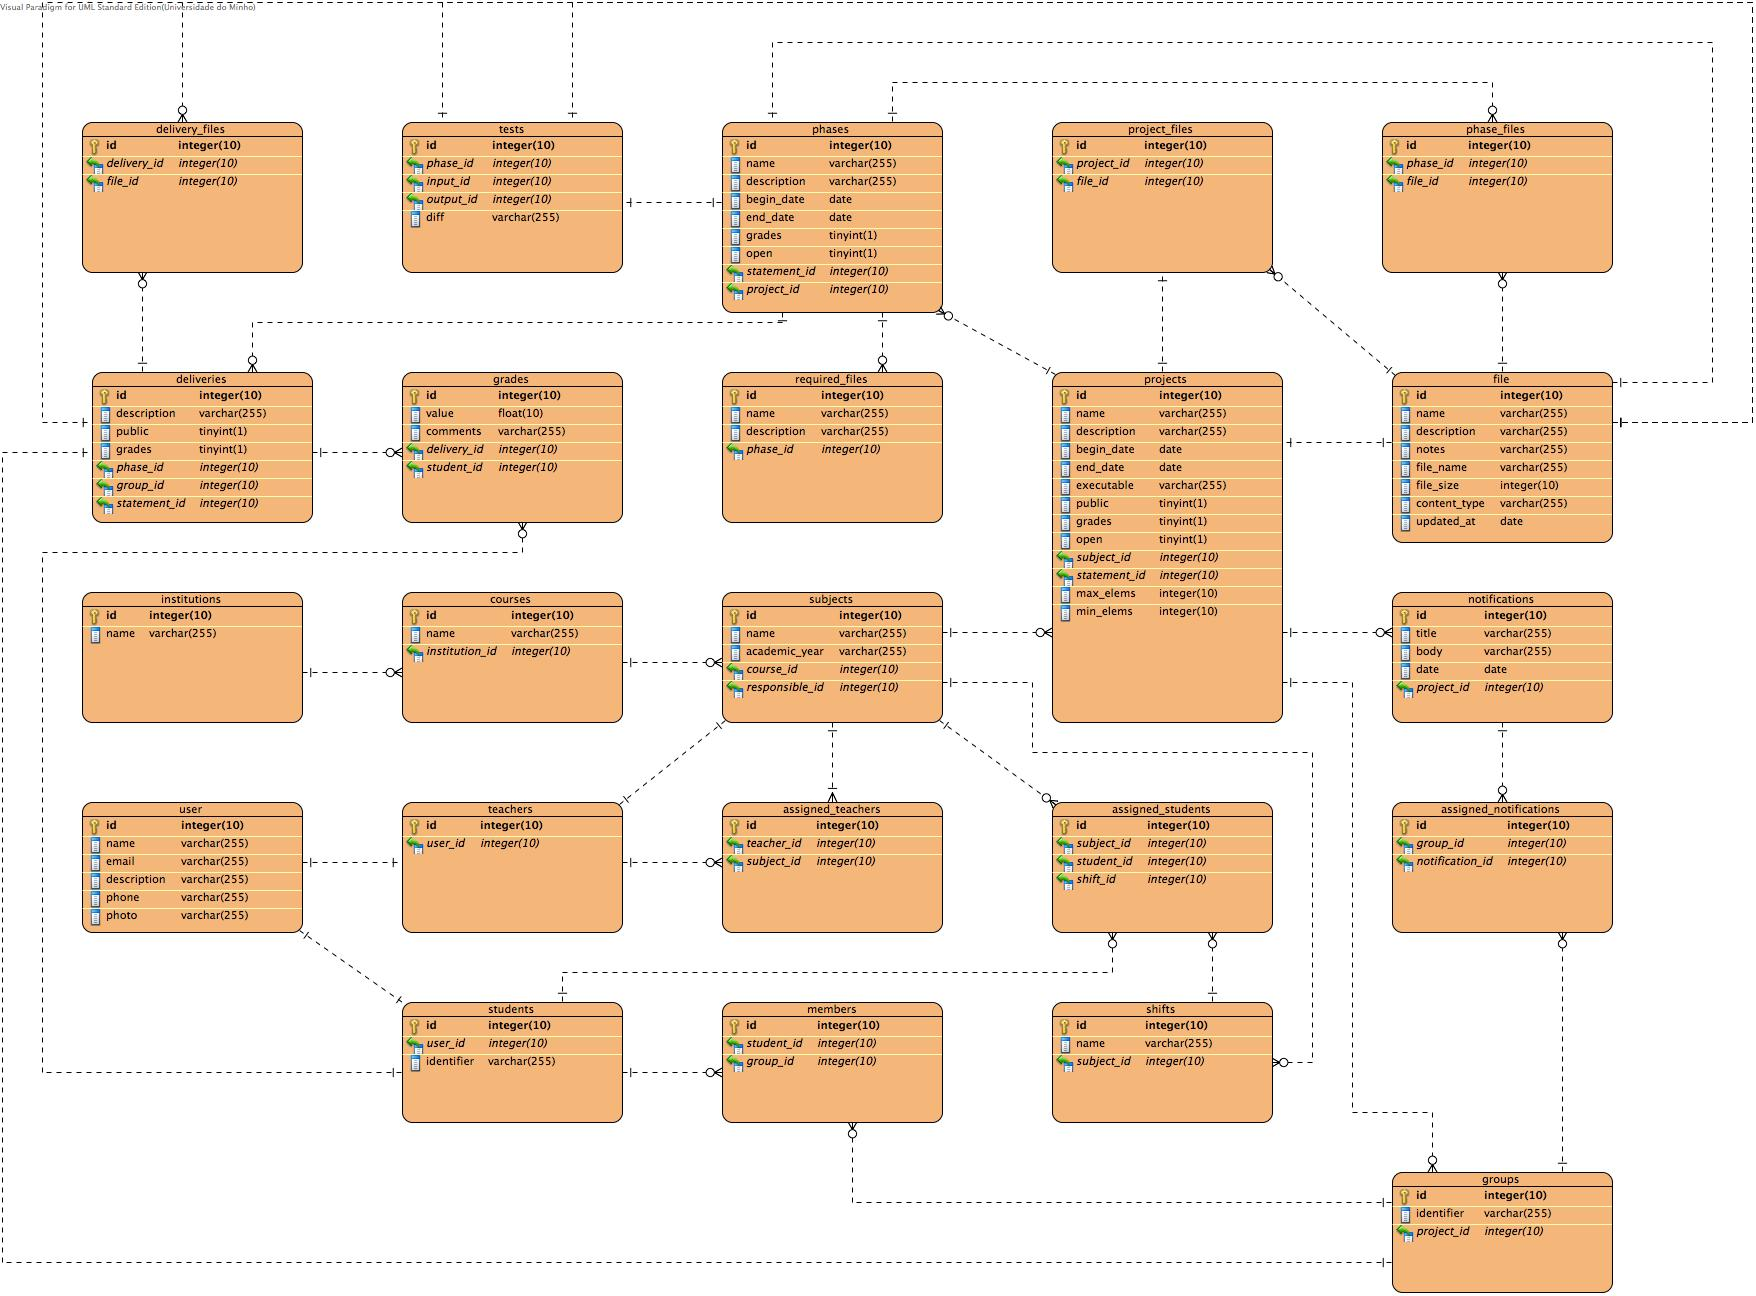
\includegraphics[width=1\textwidth,center]{images/repositorio_informacao/der}
  \caption{Diagrama Entidade Relacionamento}
  \label{fig:der}
\end{figure}

De notar que será utilizado \textbf{SQLite} em ambientes de desenvolvimento e testes, e \textbf{PostgreSQL} para ambientes de produção.

\newpage